\section{Materials and Methods}

\subsection{Polytope representation of the feasible activation space}



\subsection{Hit-and-Run}
The boundaries of the convex polytope defining the feasible activation set are defined by the mechanics of the limb and the constraints of the task, as is described in Subsection \ref{ss:finger}. The goal of the Hit-and-Run algorithm is to uniformly sample  a convex body $K$ \cite{smith1984efficient}. 
In the case of a schematic tendon-driven limb with three muscles, the feasible activations start out being the positive unit cube (as muscles can only be activated positively from 0 to a maximal normalized value of 1). As explained in \cite{Valero-Cuevas2009mathematical}, that the feasible activation set for a given static force vector produced at the endpoint of the limb is further reduced by the addition of task constraints  in the form of equality or inequality constraints that define the direction and desired magnitude of the force. Thus if this simple limb is meeting one equality constraint, the feasible activation set os the polygon $P$ containing all feasible activation  $\textbf{a} \in \mathbb{R}^n$ that satisfy
\[\textbf{f} = A\textbf{a}, \textbf{a} \in [0,1]^n,\]
where $\textbf{f} \in \mathbb{R}^m$ is a fixed force vector and $A = J^{-T}RF_m \in \mathbb{R}^{m \times n}$---the matrices of the Jacobian of the limb, the moment arms of the tendons, and the strengths of the muscles, respectively \cite{Valero-Cuevas1998Large}. $P$ is bounded by the unit $n$-cube since all variables $a_i$, $i \in [n]$ are bounded by 0 and 1 from below, above respectively.
Consider the following $1 \times 3$ fabricated example.
\begin{align*}
&1 = \frac{10}{3}a_1 - \frac{53}{15}a_2 + 2a_3 \\
&a_1, a_2, a_3 \in [0,1],
\end{align*}
the set of feasible activations is given by the shaded set in Figure \ref{fig_hr}.

\begin{figure}[ht]
   \begin{center}
    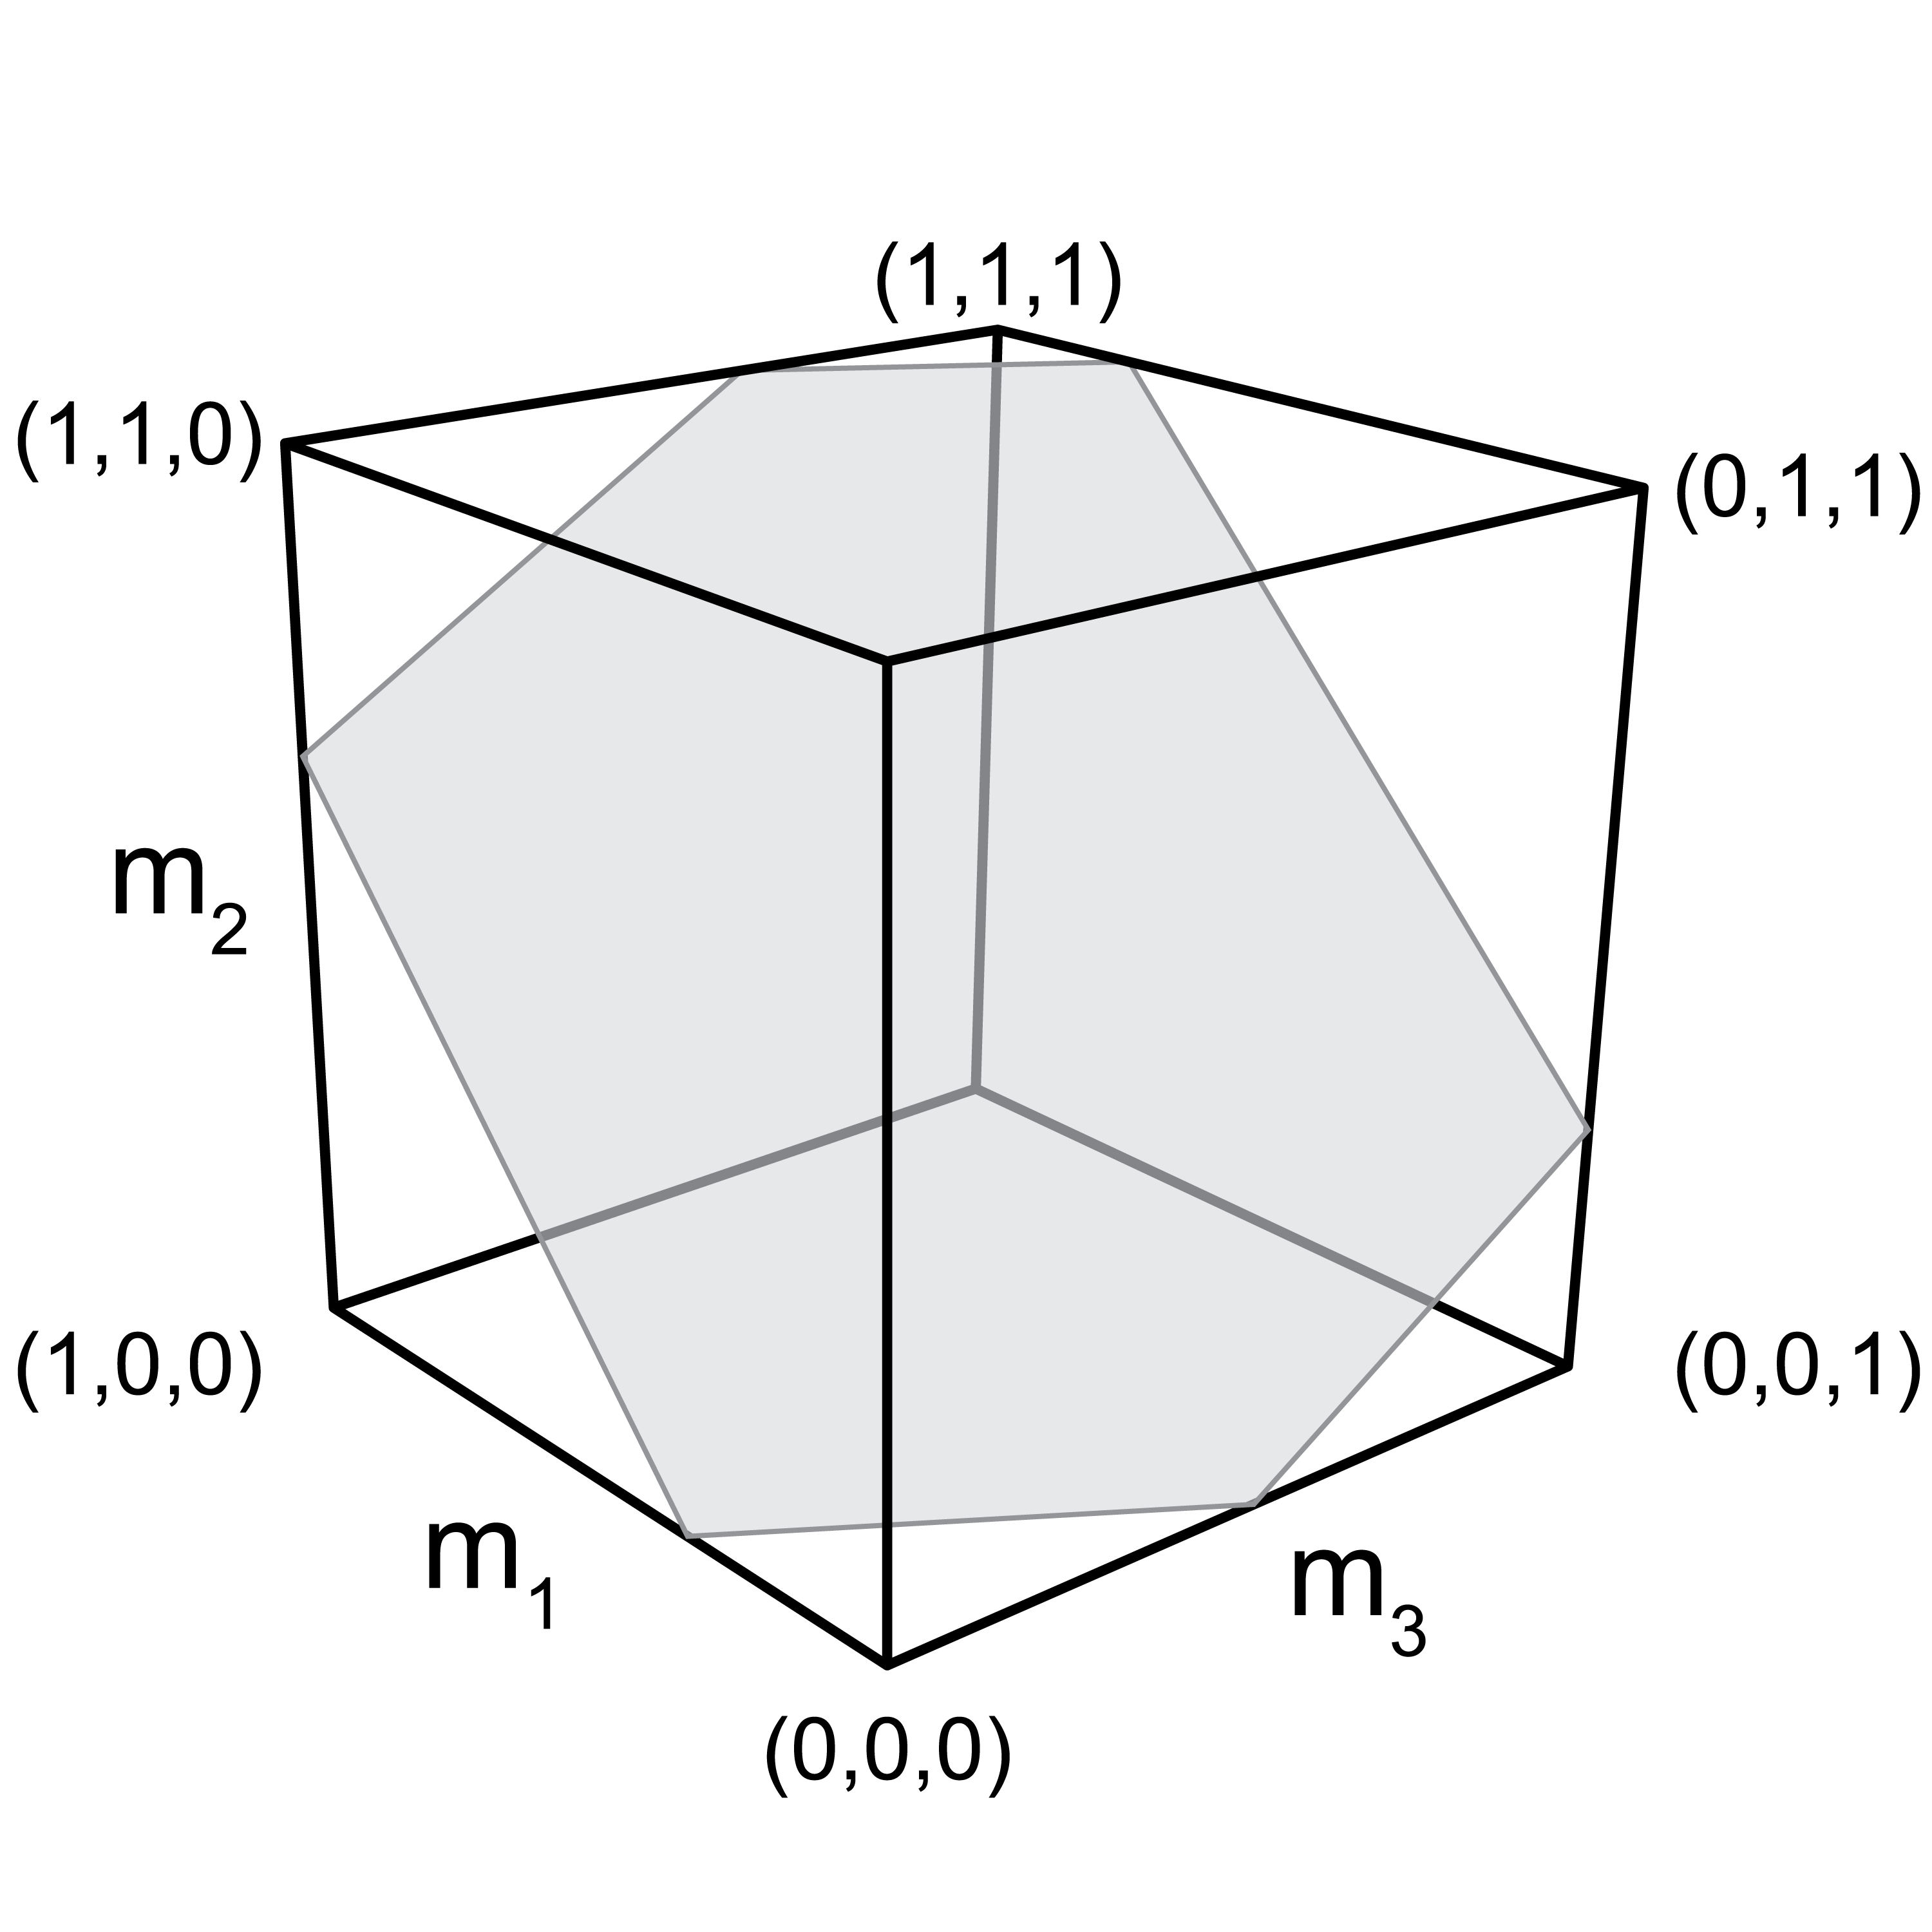
\includegraphics[width=0.25\textwidth]{sections/figs/feasibleactivation.png}
  \end{center}
  \caption{Feasible Activation}
  \label{fig_hr}
\end{figure}

The Hit-and-Run walk on $P$ is defined as follows (it works analogously for any convex body). 
\begin{enumerate}
\item Find a given starting point $\textbf{p}$ of $P$ (Figure \ref{fig_hr1}) .
\item Generate a random direction through $\textbf{p}$ (uniformly at random over all directions) (Figure \ref{fig_hr2}).
\item Find the intersection points of the random direction with the $n$-unit cube (Figure \ref{fig_hr3}).
\item Choose the next point of the sampling algorithm uniformly at random from the segment of the line in $P$ (Figure \ref{fig_hr4}). 
\item Repeat from $(b)$ the above steps with the new point as the starting point .
\end{enumerate}


\begin{figure}
        \centering
        \begin{subfigure}[b]{0.25\textwidth}
                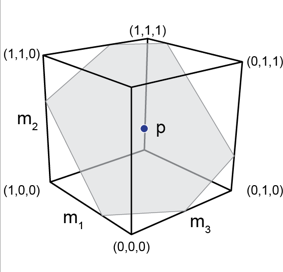
\includegraphics[width=\textwidth]{HR2.png}
                 \caption{Inner Point}
      						\label{fig_hr1}
        \end{subfigure} \hspace{0.5cm}
        \begin{subfigure}[b]{0.25\textwidth}
                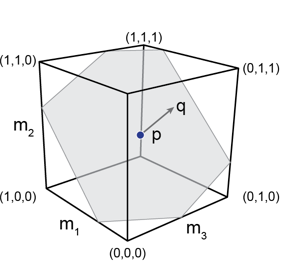
\includegraphics[width=\textwidth]{HR3.png}
                \caption{Direction}
      					\label{fig_hr2}
        \end{subfigure} \\
        \begin{subfigure}[b]{0.25\textwidth}
                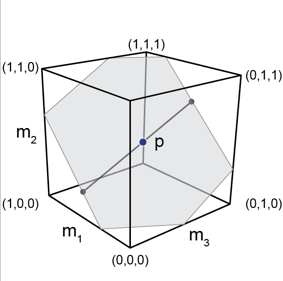
\includegraphics[width=\textwidth]{HR4.png}
                 \caption{Endpoints}
      					\label{fig_hr3}
        \end{subfigure} \hspace{0.5cm}
        \begin{subfigure}[b]{0.25\textwidth}
                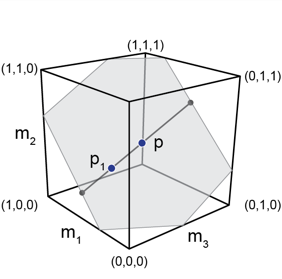
\includegraphics[width=\textwidth]{HR5.png}
                \caption{New Point}
      				 \label{fig_hr4}
        \end{subfigure}
        \caption{Hit-and-Run Step}\label{fig:animals}
\end{figure}

%\begin{figure}[ht]
%   \begin{center}
%    \includegraphics[width=0.25\textwidth]{HR1.png}
%      \caption{Inner Point}
%      \label{fig_hr1}
%    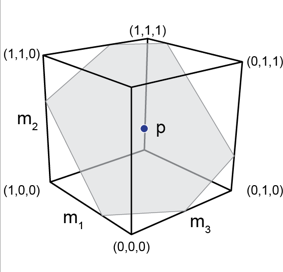
\includegraphics[width=0.25\textwidth]{HR2.png}
%    \caption{Direction}
%      \label{fig_hr2}
%    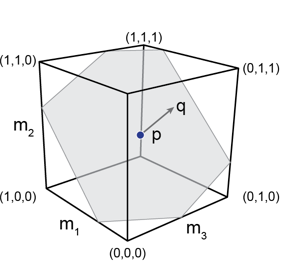
\includegraphics[width=0.25\textwidth]{HR3.png}
%    \caption{Endpoints}
%      \label{fig_hr3}
%    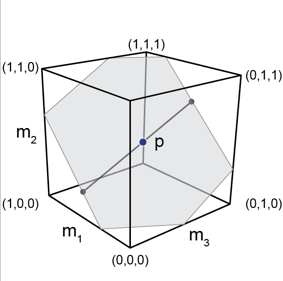
\includegraphics[width=0.25\textwidth]{HR4.png}
%    \caption{New Point}
%      \label{fig_hr4}
%  \end{center}
%\end{figure}

\begin{figure}[ht]
   \begin{center}
    \includegraphics[width=0.25\textwidth]{uniform.png}
      \caption{Uniform Distribution}
      \label{fig_hr5}
  \end{center}
\end{figure}


The implementation of this algorithm is straight forward except for the choice of the random direction. How do we sample uniformly at random (u.a.r.) from all directions in $P$? Suppose that $\textbf{q}$ is a direction in $P$ and $p \in P$. Then by definition of $P$, $\textbf{q}$ must satisfy $\textbf{f} = A(\textbf{p}+\textbf{q})$. Since $\textbf{p} \in P$, we know that $\textbf{f} = A\textbf{p}$ and therefore 
\[\textbf{f} = A(\textbf{p} + \textbf{q}) = \textbf{f} + A\textbf{q}\]
and hence
\[A\textbf{q} = 0.\]

We therefore need to choose directions uniformly at random from all directions in the vectorspace 
\[V = \{\textbf{q} \in \mathbb{R}^n | A\textbf{q} = 0\}.\]

As shown by Marsaglia this can be done as follows \cite{Marsaglia}.

\begin{enumerate}
\item
Find an orthonormal basis $b_1, \dots, b_r \in \mathbb{R}^{n}$ of $A\textbf{q} =0$.
\item
Choose $(\lambda_1, \dots, \lambda_r) \in \mathcal{N}(0,1)^n$ (from the Gaussian distribution).
\item
$\sum_{i=1}^r \lambda_i b_i$ is a u.a.r.\ direction.
\end{enumerate}

A basis of a vectorspace $V$ is a minimal set of vectors that generate $V$, and it is orthonormal if the vectors are pairwise orthogonal (perpendicular) and have unit length. Using basic linear algebra one can find a basis for $V = \{A\textbf{q} = 0\}$ and orthogonalize it with the well known Gram-Schmidt method (for details see e.g.\ \cite{Robertson}). Note that in order to get the desired u.a.r.\ sample the basis needs to be orthonormal. For the limb case we can safely assume that the rows of $A$ are linearly independent and hence the number of basis vectors is $n-m$.



\begin{figure}
        \centering
        \begin{subfigure}[b]{0.25\textwidth}
                \includegraphics[width=\textwidth]{somebasis.png}
      \caption{Some Basis}
      \label{fig_somebasis}
              \end{subfigure} \hspace{0.5cm}
        \begin{subfigure}[b]{0.25\textwidth}
                \includegraphics[width=\textwidth]{orthobasis.png}
     \caption{Direction}
      \label{Orthonormal Basis}        
      \end{subfigure}
      \caption{Find Orthonormal Basis}\label{fig_basis} 
\end{figure}


\subsection{Mixing Time}
How many steps are necessary to reach a uniformly at random point in the polytope? The theoretical bound $\mathcal{O}^*(n^2R^2/r^2)$ given in \cite{Lovasz} has a very large hidden coefficient ($10^30$) which makes the algorithm almost infeasible in lower dimensions.

These bounds hold for general convex sets. For convex polygons in higher dimensions, experimental results suggest that $\mathcal{O}(n)$ steps of the Hit-and-Run algorithm are sufficient. In particular Emiris and Fisikopoulos paper suggest that $(10 + 10\frac{n})n$ steps are enough to have a close to uniform distribution \cite{Emiris}. In all cases tested, sampling more point did not make accuarcy significantly higher. 

Ge et al.\ showed experimentally that up to about 40 dimensions, ??? random points seem to suffice to get a close to uniform discussion \cite{Ge}. 

Therfore for given output force we execute the Hit-and-Run algorithm 1000 times on 100 points. The experimental results propose that those 1000 points are uniformly distributed on the polygon.

As a additional control, for each muscle we observe that the theoretical upper and lower bound of the feasible activation match the observed corresponding bounds (difference max ??). To find the theoretical upperbound (lowerbound) of a given muscle activation we solve two linear programs maximizing (minimizing)  $a_i$ over the polytope.


%For the upper and lower bounds of the activation we can solve two linear program for each coordinate of $\textbf{a}$ to find the upper and lower bounds of each $a_i$.
%We see that those theoretical bounds match the experimentally obtained bounds.

\subsection{Starting Point}
To find a starting point in 
\[\textbf{f} = A\textbf{a}, \textbf{a} \in [0,1]^n,\]
we only need to find a feasible activation vector. For the hit and run algorithm to mix faster, we do not want the starting point to be in a vertex of the activation space. We use the following standard trick using slack variables $\epsilon_i$.

\begin{equation}\label{eq:LP_r}
\begin{array}{lrcl}
\mbox{maximize} & \sum_{i=1}^n \epsilon_i \\ 
\mbox{subject to} & \textbf{f} &=& A\textbf{a}\\
  & a_i &\in& [\epsilon_i, 1- \epsilon_i], \hspace{5mm} \forall i \in \{1,\dots,n\}  \\
  & \epsilon_i &\geq& 0, \hspace{5mm} \forall i \in \{1,\dots,n\}.  
\end{array}
\end{equation}

This approach can still fail in theory, but this method has the choose $\epsilon_i > 0$ and therefore $a_i \neq 0$ or $1$. Since for all vertices of the feasible activation space lie on the boundary of the $n$-cube, at least $n-m$ muscles must have activation $0$ or $1$. Documentation is included in our supplementary information, and all code is available at [Journal Link].

First, we first describe the stochastic method of hit-and-run, and illustrate how it functions on our fabricated 3-muscle, 1-DOF system with a desired force output of 1N.


% TODO Insert the A matrix, ith full muscle names
% Table X. Each column represents a wrench generators (with each dimension in Newtons). The muscle is modeled such that full activation would produce the column of forces and torque at the fingertip.


\subsection{Realistic index finger model}
\label{ss:finger}
We began with an index finger of a healthy human (male) right hand, which was taken from [JOB 1998]. The hand size, finger lengths, and weight was []. Experimental forces from []. 
The moment arm matrix, $R$, which contains the leverage of each tendon's insertion points across each joint, was measured by doing [], [] ,and then [].
The Jacobian, $J$, which represents the effect of rotation at each DOF on each component of endpoint wrench [cite jacobian usage], was measured with a [], by [], with precision of $\pm x$.
The force-naught vector, $F_0$, which contains the tendon force at maximal isometric contration (MIC)[cite method used] for each muscle, was taken in the [same or different] posture, with a [] measuring device, with precision of $\pm x$.


